% replace all text with your own text.
% in this template few examples are mention
\chapter{Methodology}
\label{ch:method} % Label for method chapter

\section{Importing the necessary libraries}

Importing the required Python libraries used for machine learning tasks and training models is the first step in any data processing task. These libraries facilitate various functionalities like visualization process, data manipulation, data modification, statistical analysis, training and testing of various deep learning models, and other machine learning tasks. Python has various external and built-in libraries that can be imported into the Jupyter Notebook. The libraries used for credit card fraud detection systems are as follows -

\subsection{Pandas}
Pandas is a powerful Python package made for analysis and data manipulation. It makes structured data processing simple by offering data structures like DataFrames. Pandas make it easy to effectively carry out operations like data cleansing, modification, data aggregation, data visualization, and data exploration.

\subsection{Numpy}
Numpy is a free Python software package that is intended for numerical operations on data in the form of arrays and multi-dimensional arrays. It provides standard mathematical techniques for data manipulation using linear algebra and gives users a variety of tools to manage such arrays and perform statistical operations. Basic array operations made possible by NumPy include indexing, slicing, adding, multiplying, and reshaping arrays.

\subsection{Matplotlib}
Matplotlib is a  Python data visualization package that offers a wide range of data visualization tools and functions that make data reading easy. A variety of graph types, including scatterplots, pie charts, bars, and histograms are available. Furthermore, these graphs may be exported in JPEG or PNG formats

\subsection{Seaborn}
Seaborn is one the best data visualization libraries used in Python and is a higher version of Matplotlib. It facilitates various functions and methods that can operate in data frames to perform the statistical plotting of graphs like heatmaps and histograms. Various graphs provided by this library include bar charts, histograms, error charts, scatterplots, and also heat maps which are not available in Matplotlib. It also has a feature that can select the colors that can disclose the underlying patterns and trends in the data.

\subsection{Scikit-learn}
This Python library is available as open-source and is used to build various machine learning methods. To train different machine learning methods and deep learning models, such as decision trees, support vector machines (SVM), naive Bayes, and classifiers, It also provides a variety of classification, regression, clustering, supervised and unsupervised techniques. By determining the accuracy score and producing the classification report, it also aids in evaluating the trained model's correctness; nevertheless, it cannot execute neural network models.

\subsection{Xgboost}
XGBoost, also referred to as Extreme Gradient Boost is a powerful Python module in which regression and classification are commonly used tasks. Gradient boosting methods are used by XGBoost, which is well-known for its efficiency, scalability, and operational strength. To correct mistakes produced by earlier models, these algorithms successively train inadequate learners, which are usually decision trees. Performance and utilization of resources are optimized by the library through the use of distributed and concurrent computing techniques.

\section{Data Collection}
The dataset for the credit card fraud detection system is taken from an online source Kaggle. It contains details of transactions made by the credit card by the card holders that happened in 2 days. The data set consists of 31 columns which contain the results of the transformation by PCA as numerical data input. Namely V1, V2, V3….V28 are the primary components identified by PCA. Only 2 columns which are ‘Time’ and ‘Amount’ have not undergone PCA transformation. The ‘Time’ column contains the seconds passed between each transaction and the dataset’s initial transaction. The column name ‘Amount’ contains the transaction amount which may be utilized for cost-sensitive learning based on examples. The ‘Class’ column is the answer variable and has the response as 1 in the event of fraud and 0 if no fraud is identified. It is advisable to use the Area Under the Precision-Recall Curve (AUPRC) to measure the accuracy for class imbalance ratio whereas for imbalance class, accuracy by confusion matrix is meaningless.

\begin{figure}[ht]
    \centering
    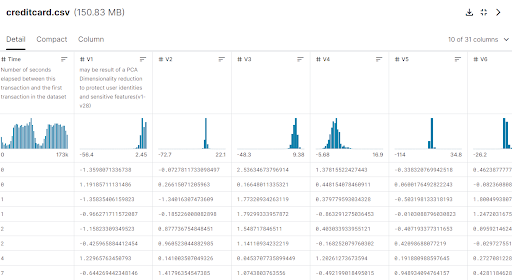
\includegraphics[scale=0.8]{figures/Data collection.png}
    \caption{Data Collection}
    \label{fig: Data Collection}
\end{figure}
.\clearpage
\section{Reading the Dataset}
Reading the Dataset is the next step after collecting the data set which is used to analyze the fraud in online transactions through credit cards. It is crucial to read the dataset after importing the required libraries to comprehend the data that has been provided. This makes it easier to train, analyze, and visualize the model of the dataset. The dataset is read by loading the CSV file into a Pandas data frame using the pd.read\_csv() function. This may be accomplished by giving the user the complete path to the CSV file or just the path to the directory in the Python environment where the dataset is uploaded. Once the dataset has been imported, data exploration is carried out. To provide an overview of the data, the top few columns and their contents are shown using the df.head() method. Here, df.head(5) provides the details of the top 5 rows and columns 


\begin{figure}[ht]
    \centering
    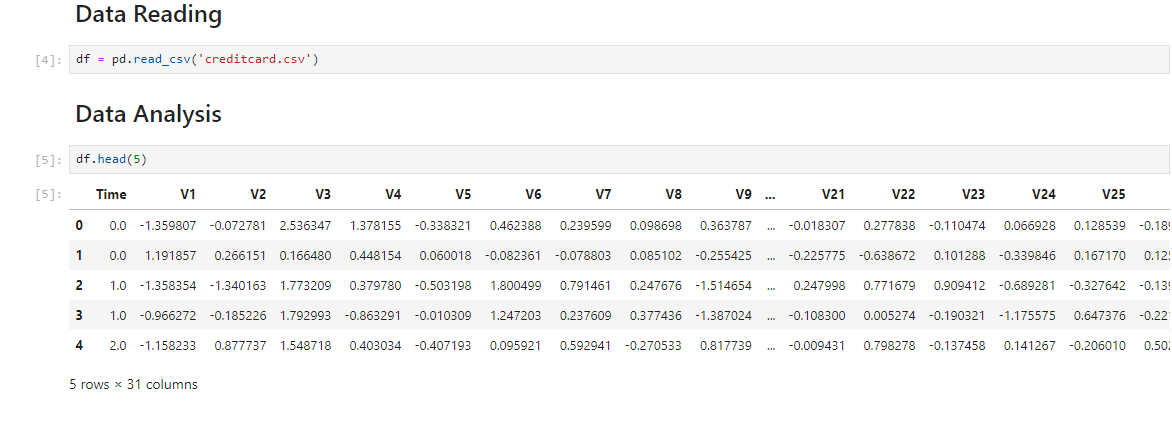
\includegraphics[scale=1]{figures/Data Reading.png}
    \caption{Fraudulent Transactions}
    \label{fig:Data Preprocessing}
\end{figure}


\section{Data Analysis}
The following step after reading the data set is to examine the substance of the data by analyzing it once the dataset has been loaded and processed in the Notebook. It entails cleansing the data by eliminating irrelevant or undesired information and handling outliers and missing numbers. After the data has been imported and cleaned, data analysis is completed. This involves examining, sanitizing, and altering the data to extract valuable insights, draw conclusions, and facilitate decision-making. Gaining understanding, making forecasts, or just working towards a particular problem's solution are all aided by data analysis. 

\begin{figure}[ht]
    \centering
    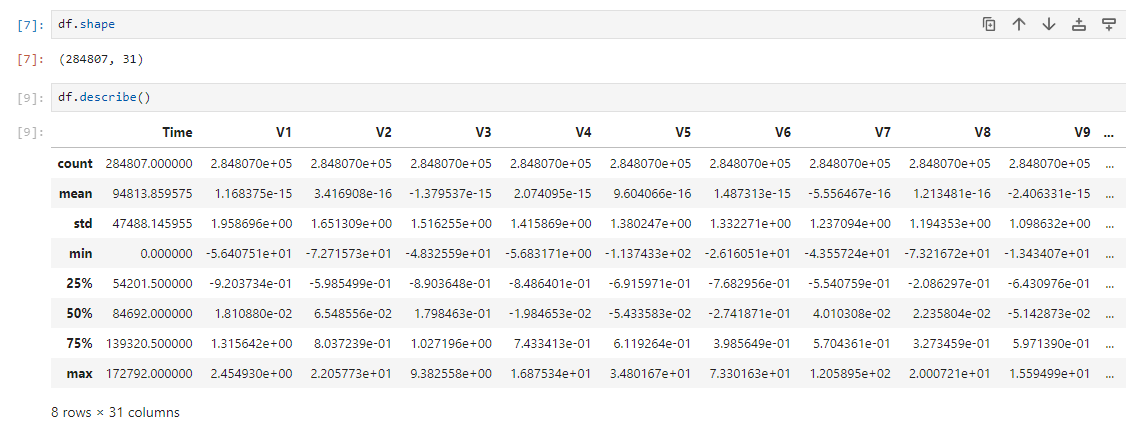
\includegraphics[scale=1]{figures/Data Analysis.png}
    \caption{Fraudulent Transactions}
    \label{fig:Data Preprocessing}
\end{figure}
\clearpage
Here, df.info() is used to get the information of the data frame which includes the data index, column name, non-null values, and the data type of that attribute. Then df.shape() is used to return the size or dimension of the data frame which is represented as the number of rows and columns. The result shows that the shape of the data frame is (284,807, 31) which denotes 284,807 rows and 31 columns. Similarly, df.describe() describes the data present in the data frame which helps to calculate statistical values like mean, median, etc. of the numerical values present in the provided data frame.


\section{Data Processing}
While processing the data set, the raw, unstructured data set is transformed into a clear, understandable form. Data pre-processing the the process of changing the data into relevant and appropriate forms before sending the data for training and testing. In this way, if the raw data contains any outliers, noise, missing values, or any irrelevant information, it can be removed before passing the data as input for the model which is the final data set. There are several  categories into which data preparation techniques are divided. Detecting outliers and addressing missing numbers are the two primary tasks of this phase. Various cleaning procedures are done to clean the data set by addressing problems which include noisy data, missing values, finding and removing outliers, and solving the differences. If users believe that the data is polluted, they are less inclined to trust data mining results. Values for a characteristic that differs from other data by more than two standard deviations might be classified as outliers. 
\begin{lstlisting}[language=Python, caption={Creating and training Catboost model}, label=list:python_code_ex]
#check if there any duplication
df.duplicated().sum()
1081

 # drop duplication data

df.drop_duplicates(inplace=True)
\end{lstlisting}

The process of data visualization is crucial to data analysis and investigation. The data visualization is supported by several built-in libraries in Python. This method presents the data in a highly graphical manner that facilitates better visual comprehension of the information, making it simpler to analyze trends and recognize patterns and correlations between several variables. Several graphs may be drawn, and each kind of graph depicts the data uniquely. The two Python libraries that are most frequently utilized when importing the graphical representation are Matplotlib and Seaborn. Many graph formats, including line, scatter, bar, and histogram plots, are supported by Matplotlib. However, Seaborn is based on Matplotlib and is an improved version of it. 

Checking for any missing values is done using the df.isna() function. Then, the data is processed for any duplicate values if present using the df.duplicates(). The result shows that there are 1081 duplicate values present in the dataset. These duplicate values are removed or dropped using the df.drop() function.

The given dataset contains the time and date of the transaction which can be used to determine the cases of fraud and valid transactions. The given data is plotted in a pie graph to visually represent the percentage of valid or legitimate transactions made with the credit card which is denoted as ‘0’ while the percentage of fraud transactions is denoted as ‘1’. The green part of the pie chart shows that ‘0’ i.e. the percentage of cases of legitimate transactions is 99.83\% while the red part of the pie chart displays the percentage of cases of fraud transactions which is 0.17\%. This data can simplify the process of identifying fraudulent transactions which helps financial institutions, and credit card owners from any fraudulent activities and transactions.


\begin{figure}[ht]
    \centering
    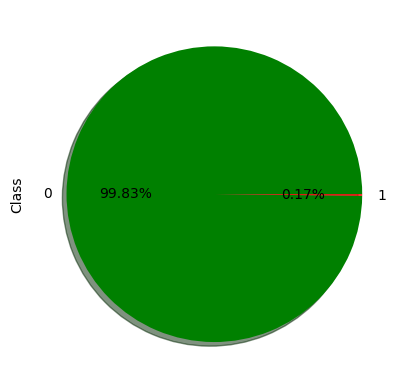
\includegraphics[scale=1]{figures/Preprocessing.png}
    \caption{Fraudulent Transactions}
    \label{fig:Data Preprocessing}
\end{figure}


\clearpage

 \section{Training and Test Split}
 After the data processing of the given dataset which includes cleaning and visualizing the data, the next step is to divide the data set into training and testing data which is used to train the deep learning model. Dividing the data set into training and testing data ensures that the model can be trained on the training part of the data and then the model can be evaluated on the testing part of the data. This can be done by using the Scikit-learn library and the data is split in such a manner that around 80\% of the data is used for the training part i.e.\textbf{ x\_train }\& \textbf{y\_train }while the remaining 20\% of the data is used for the testing i.e. \textbf{x\_test }\&\textbf{ y\_test} and evaluation part. This ensures that the data is appropriately distributed for the model to learn effectively and generate accurate predictions. Also, splitting the dataset helps to avoid overfitting issues in which the model can strongly perform on training data but poorly on new data ensuring the establishment of a robust credit card fraud detection system that works effectively in the real world.

\begin{lstlisting}[language=Python, caption={Creating and training Catboost model}, label=list:python_code_ex]
# Spliting the data into X and Y
X = df.drop(columns="Class")
y = df["Class"]

# Spliting the data into training and testing set
X_train, X_test, y_train, y_test = train_test_split(X, y, test_size=0.25, random_state=42)


# checking shape of training and testing set
print("X Train : ", X_train.shape)
print("X Test  : ", X_test.shape)
print("Y Train : ", y_train.shape)
print("Y Test  : ", y_test.shape)
\end{lstlisting}

 \section{Data Oversampling Handling}
Oversampling of data needs to be handled to increase the efficiency and quality of the sample data. One such technique to handle oversampling of data is the Synthetic Minority Over-sampling Technique (SMOTE) which is crucial to enhance the performance of the model. When the data proportion of valid transactions is comparatively larger than the fraud transaction, SMOTE helps to balance the distribution of such imbalanced data by creating data points for the minority class. In this process, new instances of the data are created using the data that is already present to improve the model’s accuracy in identifying and detecting fraud transactions.SMOTE also reduces the chance of overfitting while simultaneously increasing the size of the data set. In cases like credit card fraud detection, where even minute errors can have a huge impact or loss for the specific financial institutions. Using such an approach to handle the oversampling of data is a preventive action that strengthens the sensitivity and performance of the machine learning models that are deployed.

\begin{lstlisting}[language=Python, caption={Creating and training Catboost model}, label=list:python_code_ex]
# Apply SMOTE for solving sampling problem
smote = SMOTE(random_state=42)
X_resampled, y_resampled = smote.fit_resample(X_train, y_train)
\end{lstlisting}

 
 



\section{Implementation}
\subsection{Logistic Regression}
 Logistic Regression is a method where an outcome is determined by one or more distinct variables that may be analyzed statistically and are used to address binary classification issues and are applied in various domains like machine learning. Because of its ease of use and efficiency in forecasting the likelihood of fraudulent transactions, logistic regression can be very useful in detecting credit card fraud. Logistic Regression works by setting a specific threshold, this approach transforms the output into a probability score that falls between 0 and 1. This score can subsequently be categorized into one of two binary options: either fraud or not fraud. This method can be implemented by the Scikit-learn library by first creating the model using the \textbf{LogisticRegression()} function and then training the model with the training data x\_train and y\_train.

\begin{lstlisting}[language=Python, caption={Code snippet in \LaTeX ~and  this is a Python code example}, label=list:python_code_ex]
model = LogisticRegression()

# Training the model
model.fit(X_resampled, y_resampled)
\end{lstlisting}
 

 
After training the model, the testing set of output is predicted and the performance of the model is evaluated based on various evaluation metrics like the confusion matrix, accuracy score and the F1 score. However, the F1 Score is more reliable than the accuracy score as we are dealing with anomalies in the data which means there might be very few cases of fraud transactions out of many transactions which is a case of data imbalance. The accuracy score of the Logistic Regression model is 0.9778 and the F1 Score is 0.55075. A Confusion matrix is also plotted which shows the actual values and predicted values. 





\begin{figure}[ht]
    \centering
    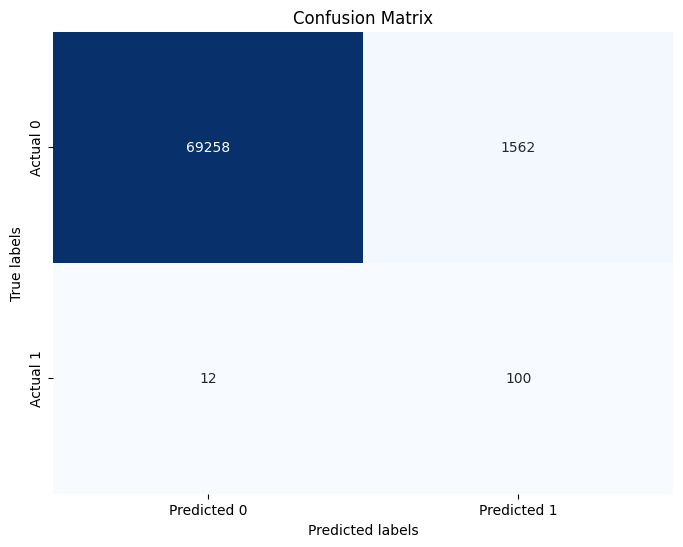
\includegraphics[scale=0.7]{figures/CM_LogisticRegression.png}
    \caption{Figure of the Data}
    \label{fig:Plot of the Data}
\end{figure}



\subsection{Grid Search Logistic Regression}

Grid search is a popular machine learning technique that goes through different values of parameters and then selects the best out of them. It is a hyperparameter tuning technique that is used to find the best parameter for a specific model. In this research, grid search is implemented along with the logistic regression model which is very essential for predicting fraud transactions in credit cards. Grid search in logistic regression is a systematic approach to assess model performance over a given grid of hyperparameters which contributes to this process by helping the logistic regression model be adjusted to achieve the ideal ratio of the difference to bias, improving the model's capacity to correctly identify fraudulent transactions. It also helps choose the best configuration by providing information on how various hyperparameters affect the performance of the model. 

\begin{lstlisting}[language=Python, caption={Code snippet in \LaTeX ~and  this is a Python code example}, label=list:python_code_ex]
# Define the logistic regression model
logistic_regression = LogisticRegression()

# Define hyperparameters to tune
param_grid = {
    'C': [0.001, 0.01, 0.1, 1, 10, 100],  # Regularization parameter
    'penalty': ['l1', 'l2']                # Penalty term
}

# Perform grid search with 5-fold cross-validation
grid_search = GridSearchCV(estimator=logistic_regression, param_grid=param_grid, cv=5, scoring='f1_macro', verbose=1)

# Fit the grid search to the data
grid_search.fit(X_resampled, y_resampled)

# Get the best parameters
best_params = grid_search.best_params_
print("Best Parameters:", best_params)

# Train the logistic regression model with the best parameters
best_model = LogisticRegression(**best_params)
best_model.fit(X_resampled, y_resampled)
\end{lstlisting}

\begin{figure}[ht]
    \centering
    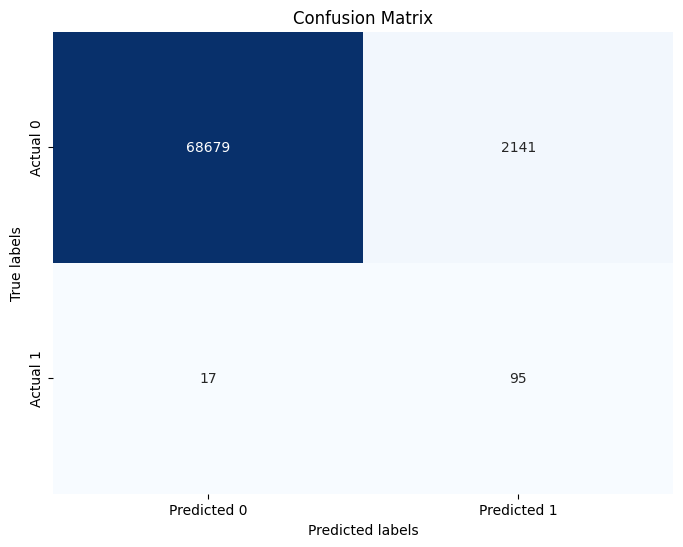
\includegraphics[scale=0.9]{figures/CM_GridSearch.png}
    \caption{Figure of the Data}
    \label{fig:Plot of the Data}
\end{figure}

\clearpage


\subsection{Random Forest Classification}

Random Forest classification is an improved version of the decision tree methodology which uses a forest made up of many trees and combines the outcome or predictions of each tree. In this forest, each tree is built using a random subset of the training dataset. This technique helps to reduce the chances of overfitting by lowering the variation of the model which is often encountered in the decision tree. The Random Forest approach produces a more accurate and dependable model when it comes to credit card fraud detection since it can handle the complicated and irregular trends in the data. The classifier is initiated by using the function \textbf{RandomForestClassifier() }and then training the classifier using the training data i.e. x\_train and y\_train. Random Forest’s ability to forecast is improved by using an ensemble approach, which allows it to recognize a wide range of fraud indications distributed over several trees. The flexibility of Random Forest to provide relevance ratings to individual features makes it a helpful  tool for identifying the primary factors influencing fraud alarms, despite its complexity and higher processing requirements compared to Decision Trees.

\begin{lstlisting}[language=Python, caption={Code snippet in \LaTeX ~and  this is a Python code example}, label=list:python_code_ex]
# Defining the Random Forest classifier
random_forest_classifier = RandomForestClassifier(n_estimators=100, random_state=42)

# Trainining the Random Forest classifier
random_forest_classifier.fit(X_resampled, y_resampled)
\end{lstlisting}


\clearpage

 After training the model, the performance of the model is evaluated based on various evaluation metrics like the confusion matrix, accuracy score and the F1 score. However, the F1 Score is more reliable than the accuracy score as we are dealing with anomalies in the data which means there might be very few cases of fraud transactions out of many transactions. The accuracy score of the Random Forest Classifier model is 0.9995 and the F1 Score is 0.9257. A Confusion matrix is also plotted which shows the actual values and predicted values.


 \begin{figure}[ht]
    \centering
    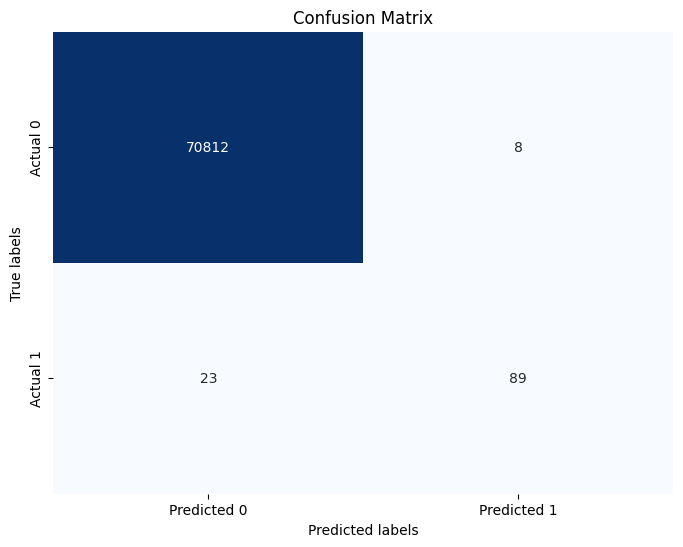
\includegraphics[scale=0.7]{figures/CM_RandomForest.png}
    \caption{Figure of the Data}
    \label{fig:Plot of the Data}
\end{figure}



 \subsection{eXtreme Gradient Boost }

 XG Boost or Extreme Gradient Boosting is a complex variant of the gradient boosting method that is recommended for its quick processing speed and outstanding effectiveness. To optimize the utilization of computing resources and raise the overall effectiveness of models, it provides a flexible and accurate method for improving decision tree models. When the number of fraud transactions is much more than the number of valid transactions, then data imbalance occurs which can be resolved by using XGBoost. To do this, it uses a gradient boosting framework, which sequentially and cautiously fixes flaws from previous models (trees). With a technique called boosting, every succeeding model seeks to gradually reduce the errors found in its earlier models.XGBoost is a helpful tool for identifying complex fraudulent behaviour in large transactional data sets due to its capacity to handle minimal data, work with a variety of loss functions, and analyze inaccurate information instantly. 
\clearpage

 \begin{lstlisting}[language=Python, caption={Code snippet in \LaTeX ~and  this is a Python code example}, label=list:python_code_ex]
# Initializing the XGBoost model
xg = xgb.XGBClassifier()

# Training the XGBoost model
xg.fit(X_resampled, y_resampled)
y_pred = xg.predict(X_test)

# Calculating AUC Curve for XGBoost
y_pred_probability = xg.predict_proba(X_test)[::,1]
fpr, tpr, _ = metrics.roc_curve(y_test, y_pred_probability)
auc = metrics.roc_auc_score(y_test, y_pred_probability)
plt.plot(fpr,tpr,label="XGBoost, auc="+str(auc))
plt.legend(loc=4)
plt.show()
\end{lstlisting}


 An important assessment indicator is the AUC (Area Under the Curve) curve generated by XGBoost in a credit card fraud detection system. This curve shows how well the model can distinguish between fraudulent and legitimate transactions across various parameters. The graph illustrates the relationship between the true positive and false positive rates, offering a significant understanding of the model's precision in detecting fraudulent transactions while mitigating false positives. When the AUC value approaches 1, it signifies that the model has a strong discriminating capacity and can effectively discriminate between fraudulent and legal transactions. The AUC score of this model is 0.9721. 

 

 A lower AUC value, on the other hand, that is closer to 0.5 denotes poorer model performance, similar to chance in class distinction. Because of this, the AUC value serves as a crucial metric for evaluating how successfully the model detects fraudulent activity while lowering false positives. It provides insightful information about the model's reliability and ability to predict outcomes in real-world situations. As the curve moves closer to the upper-left corner, indicating higher true positive rates and lower false positive rates, the model demonstrates increased filtering ability and reliability in differentiating between authentic and fraudulent behaviours. 


\begin{figure}[ht]
    \centering
    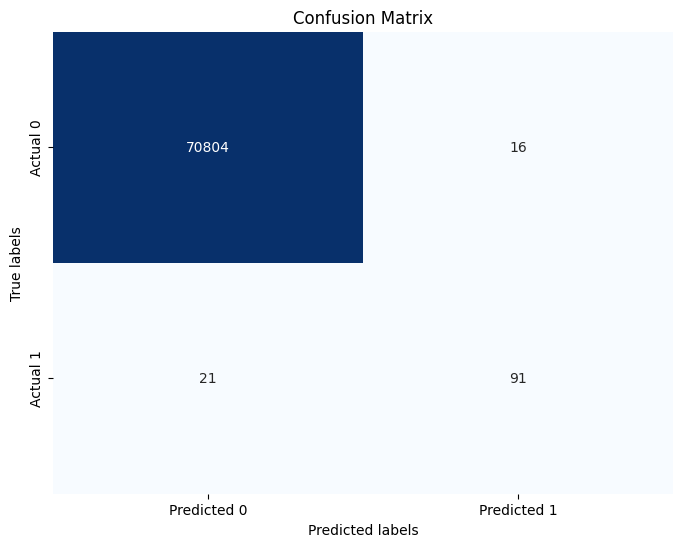
\includegraphics[scale=0.7]{figures/CM_XGBoost.png}
    \caption{Figure of the Data}
    \label{fig:Plot of the Data}
\end{figure}
 The accuracy score of the Xgboosting Classifier model is 0.9994 and the F1 Score is 0.9153 

 \begin{figure}[ht]
    \centering
    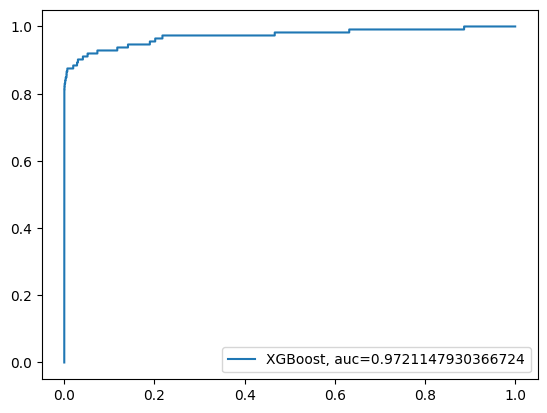
\includegraphics[scale=0.7]{figures/XGBoost.png}
    \caption{Figure of the Data}
    \label{fig:Plot of the Data}
\end{figure}

\clearpage
 \subsection{Categorical Boost}

 CatBoost, also known as Categorical Boosting is a popular machine learning approach that is built upon the gradient boosting platforms and is particularly designed to handle the categorical variables efficiently. CatBoost effectively incorporates this data to improve the recognition of fraudulent transactions in credit card fraud detection, where datasets often consist of both numerical and categorized data. CatBoost can handle the complexity of fraud detection activities with ease because of its gradient-boosting mechanism and special way of processing categorical data. This helps to prevent overfitting and maintain the highest possible accuracy. CatBoost uses a structured boosting technique to reduce the error in prediction and to provide a more accurate and reliable model. In addition, it is especially useful in complex fraud detection cases where categorization into many fraud categories is required because of its inherent capacity for multi-classification and its capacity to manage inaccurate information. Building robust and effective credit card fraud detection systems is made easier with CatBoost's versatility, ease of use, and dependability while managing a variety of data formats. The model is running for 100 iterations with a learning rate of 0.5 and the evaluation metric chosen is AUC.

 \begin{lstlisting}[language=Python, caption={Creating and training Catboost model}, label=list:python_code_ex]
# Initialize CatBoost model
cb_model = CatBoostClassifier(iterations=100,
                              depth=12,
                              eval_metric='AUC',
                              random_seed=2018,
                              od_type='Iter',
                              metric_period=1,
                              od_wait=100)

# Make predictions using the CatBoost model
cb_predict = cb_model.predict(X_test)
\end{lstlisting}
\clearpage

 The accuracy score of the Catboost Boosting Classifier model is 0.9991 and the F1 Score is 0.8769.  

\begin{figure}[ht]
    \centering
    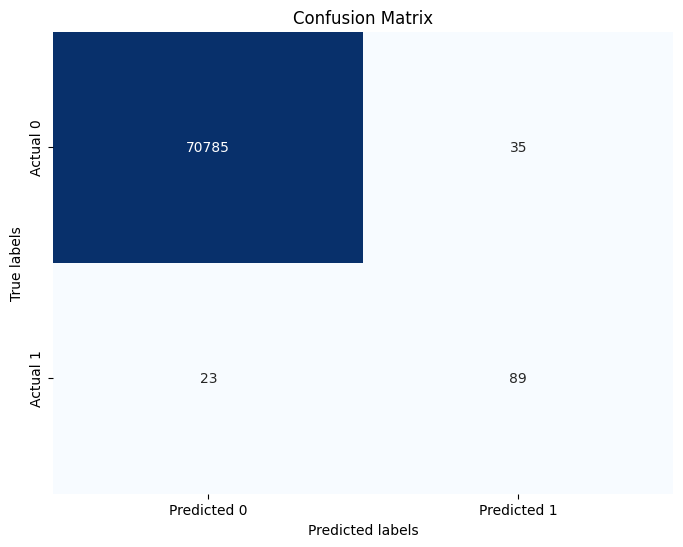
\includegraphics[scale=0.6]{figures/CM_CatBoost.png}
    \caption{Confusion Matrix}
    \label{fig:Plot of the Data}
\end{figure}

\clearpage




